\documentclass[tikz,border=10pt]{standalone}
\usepackage{tikz}
\usepackage{amsmath}

\begin{document}
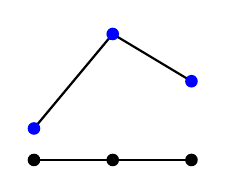
\begin{tikzpicture}[scale=2]
    % Define the vertices of the reference triangle
    \coordinate (A) at (0,0.2);
    \coordinate (B) at (0.5,0.8);
    \coordinate (C) at (1.0,0.5);


    \coordinate (N0) at (0.0,0.0);
    \coordinate (N1) at (0.5,0.0);
    \coordinate (N2) at (1.0,0.0);


    \draw[black, thick] (A) -- (B) -- (C);

    \draw[black, thick] (N0) -- (N1) -- (N2);



    \fill[blue] (A) circle (0.04);
    \fill[blue] (B) circle (0.04);
    \fill[blue] (C) circle (0.04);


    \fill[black] (N0) circle (0.04);
    \fill[black] (N1) circle (0.04);
    \fill[black] (N2) circle (0.04);

\end{tikzpicture}
\end{document}

